\documentclass[../main.tex]{subfiles}

\begin{document}
%%%%%%%%%%%%%%%%%%%%%%%%%%%%%%%%%%%%%%%%%%%%%%%
%                                             %
% Integralrechnung III -- Integrationstechnik %
%                                             %
%%%%%%%%%%%%%%%%%%%%%%%%%%%%%%%%%%%%%%%%%%%%%%%
\chapter{SW10 Integralrechnung III -- Integrationstechnik}
\section{2. Substitutionsregel}
Die 2. Substitutionsregel ist flexibler und auf beliebige Integrale anwendbar: \\ [7pt]
$\int f(x)dx$ \\ [7pt]
indem man dort $x = u(t)$ setzt und somit wegen $dx = u'(t)dt$ schreiben kann. \\ [7pt]
$\int f(x)dx = \left[ \int f(u(t))u'(t)dt \right]_{t=u^{-1}(x)}$ \\ [7pt]
u muss im verwendeten t-Intervall umkehrbar sein, damit man $x=u(t)$ nach t auflösen, dh. durch x ausdrücken kann ($t=u^{-1}(x)$).

\subsection{Theorem - 2. Substitutionsregel für unbestimmte Integrale}
Es gilt: $\int f(x)dx = \left[ \int f(u(t))u'(t)dt \right]_{t=u^{-1}(x)}$ \\ [7pt]
Vorgehen: \\
\begin{itemize}
    \item Wähle eine geeignete invertierbare Substitutionsfunktion $u$
    \item Substituiere formal $x = u(t), dx = u'(t)dt$
    \item Integriere nach $t$
    \item Drücke $t$ durch $x$ aus
\end{itemize}
\subsection{Beispiele}
Berechne $I = \int x^2 \sqrt[]{x-1}dx$ \\
$u = x-1$ \\
$x = u + 1$ \\
$\frac{du}{dx} = 1$ \\
$du = dx$ \\ [7pt]
$I = \int x^2 \sqrt[]{x-1}dx = \int (u+1)^2 \sqrt[]{u} du = \int (u^2 + 2u +1)u^{\frac{1}{2}}du$
$ = \int (u^{\frac{5}{2}} + 2u^{\frac{3}{2}} + u^{\frac{1}{2}})du$ \\ [7pt]
$ = \frac{u^{\frac{7}{2}}}{\frac{7}{2}} + \frac{u^{\frac{5}{2}}}{\frac{5}{2}} +\frac{u^{\frac{3}{2}}}{\frac{3}{2}} + C$ 
$ = \frac{2}{7}u^{\frac{7}{2}} + \frac{2}{5}u^{\frac{5}{2}} + \frac{2}{3}u^{\frac{3}{2}} + C$ \\ [7pt]
$ = (\frac{2}{7}u^{\frac{6}{2}} + \frac{2}{5}u^{\frac{4}{2}} + \frac{2}{3}u^{\frac{2}{2}})u^{\frac{1}{2}} + C$
$ = (\frac{2}{7}u^{\frac{6}{2}} + \frac{2}{5}u^{\frac{4}{2}} + \frac{2}{3}u^{\frac{2}{2}})\sqrt[]{u} + C$
$ = (\frac{2}{7}u^3 + \frac{2}{5}u^2 + \frac{2}{3}u)\sqrt[]{u} + C$ \\ [7pt]
$ = (\frac{2}{7}(x-1)^3 + \frac{2}{5}(x-1)^2 + \frac{2}{3}(x-1))\sqrt[]{(x-1)} + C$ \\ [14pt]
\noindent\rule{8cm}{0.4pt} \\
Berechne $I = \int \frac{dx}{\sqrt[]{1+e^x}}$ es werden zwei Substitutionen benötigt. \\ [7pt]
$ u = e^x$ \\
$ \frac{du}{dx}= e^x$ \\
$ du = e^xdx \Longrightarrow dx = \frac{du}{e^x} = \frac{du}{u}$ \\
$I = \int \frac{dx}{\sqrt[]{1+e^x}} = \int \frac{\frac{du}{u}}{\sqrt[]{1+u}}$
$ = \int \frac{du}{u\sqrt[]{1+u}}$ \\ [7pt]
$v = \sqrt[]{1+u}$ \\
$ v^2 = 1+u \Longrightarrow u = v^2-1$ \\
$ \frac{du}{dv} = 2v$ \\
$ du = 2vdv$ \\ [7pt]
$\int \frac{2vdv}{(v^2-1)v} = 2 \int \frac{dv}{v^2-1} = \frac{1}{2}2\log | \frac{v-1}{v+1} | + C$
$ = \log | \frac{\sqrt[]{1+u}-1}{\sqrt[]{1+u}+1}| + C = \log | \frac{\sqrt[]{1+e^x}-1}{\sqrt[]{1+e^x}+1}| + C$

\subsection{Theorem - 2. Substitutionsregel für bestimmte Integrale}
Es gilt: $ \int\limits_a^b f(x)dx = \int\limits_{u^{-1}(a)}^{u^{-1}(b)} f(u(b))u'(t)dt$ \\
Vorgehen: \\
\begin{itemize}
    \item Wähle eine geeignete invertierbare Substitutionsfunktion $u$
    \item Substituiere formal $x=u(t)$,$dx=u'(t)dt$
    \item Ersetze die $x$-Grenzen $a,b$ durch die $t$-Grenzen $u^{-1}(a),u^{-1}(b)$
    \item Integriere
\end{itemize}

\subsection{Beispiele}
Berechne $I = \int\limits_1^2 x^2\sqrt[]{x-1}dx$ \\
$t = x-1$ \\
$x = t +1$ \\
$\frac{dx}{dt} = 1$ \\
$dx = dt$ \\ [7pt]
Alte Grenzen: $a = 1, b=2$ neue Grenzen: $t(a) = 0, t(b) = 1$ \\
$ \int\limits_0^1 (t+1)^2 \sqrt[]{t}dt = \int\limits_0^1 (t^2 + 2t +1)t^{\frac{1}{2}}$
$ = \int\limits_0^1 (t^{\frac{5}{2}} + 2t^{\frac{3}{2}} + t^{\frac{1}{2}})dt$
$ = \left[ \frac{2}{7}t^{\frac{7}{2}} + \frac{4}{5}t^{\frac{5}{2}} + \frac{2}{3}t^{\frac{3}{2}}  \right]_0^1$ \\ [7pt]
$ = \frac{2}{7} + \frac{4}{5} + \frac{2}{3} - 0 = \frac{184}{105}$ \\[14pt]
\noindent\rule{8cm}{0.4pt} \\
Berechne $I = \int\limits_0^{\ln 3} \frac{dx}{\sqrt[]{1+e^x}}$ es werden zwei Substitutionen benötigt. \\
$u = e^x$ \\
$x = \ln u$ \\
$dx = \frac{1}{u}du$ \\ [7pt]
$I = \int\limits_0^{\ln 3} \frac{dx}{\sqrt[]{1+e^x}} = \int\limits_0^{\ln 3} \frac{1}{\sqrt[]{1+e^x}}dx$ \\ [7pt]
Alte Grenzen: $a=0, b=\ln 3$, neue Grenzen: $u(\ln 3) = 3, u(0) = 1$ \\ [7pt]
$\int\limits_1^3 \frac{1}{\sqrt[]{1+u}} \times \frac{1}{u}du$ \\ [7pt]
$v = \sqrt[]{1+u}$ \\
$v^2 = 1+u$ \\
$u = v^2 -1$ \\
$\frac{du}{dv} = 2v$ \\
$du = 2vdv$ \\ [7pt]
Alte Grenzen: $a=1, b=3$, neue Grenzen: $v(1) = \sqrt[]{2}, v(3) = 2$ \\ [7pt]
$\int\limits_{\sqrt[]{2}}^2 \frac{1}{v} \frac{1}{v^2-1} 2vdv$
$ = 2 \int\limits_{\sqrt[]{2}}^2 \frac{dv}{v^2-1}$
$ = 2 \left[ \frac{1}{2} \log |\frac{v-1}{v+1}| \right]_{\sqrt[]{2}}^2 \approx 0.6641  $

\section{Häufige Integralsubstitutionen}
\begin{tabularx}{0.9\textwidth} { 
    >{\centering\arraybackslash}X 
    >{\centering\arraybackslash}X  }
    \rowcolor{lightgray} A) Integraltyp & Substitution \\ [7pt]
    \hline
    $ \int f(ax + b)dx$ 
    \newline \newline
    Merkmal: Die Variable $x$ tritt in der linearen Form $ax+b$ auf ($a \neq 0$)
    &
    $ u = ax + b$
    \newline 
    $ dx = \frac{du}{a}$
    \\ [7pt]
\end{tabularx}
\\ [7pt]

\begin{tabularx}{0.9\textwidth} { 
    >{\centering\arraybackslash}X 
    >{\centering\arraybackslash}X  }
    \rowcolor{lightgray} A) Beispiele & Substitution \\ [7pt]
    \hline
    $\int (2x - 3)^6dx$ 
    &
    $u=2x-3$ 
    \\ [7pt]
    $\int \sqrt[]{4x + 5}dx$
    &
    $ u=4x+5$
    \\ [7pt]
    $ \int e^{4x+2} $
    &
    $u = 4x+2$
    \\ [7pt]
\end{tabularx}
\\ [7pt]

\begin{tabularx}{0.9\textwidth} { 
    >{\centering\arraybackslash}X 
    >{\centering\arraybackslash}X  }
    \rowcolor{lightgray} B) Integraltyp & Substitution \\ [7pt]
    \hline
    $ \int f(x)f'(x)dx$
    \newline \newline
    Merkmal: Der Integrand ist das Produkt aus einer Funktion $f(x)$ 
    und ihrer
    Ableitung $f'(x)$
    &
    $ u = f(x)$
    \newline 
    $ dx = \frac{du}{f'(x)}$
    \\ [7pt]
\end{tabularx}
\\ [7pt]

\begin{tabularx}{0.9\textwidth} { 
    >{\centering\arraybackslash}X 
    >{\centering\arraybackslash}X  }
    \rowcolor{lightgray} B) Beispiele & Substitution \\ [7pt]
    \hline
    $\int \sin (x) \cos (x) dx$ & $ u = \sin x$
    \\ [7pt]
    $\int \frac{\ln x}{x}dx$ & $u=\ln x$
    \\ [7pt]
\end{tabularx}
\\ [7pt]

\begin{tabularx}{0.9\textwidth} { 
    >{\centering\arraybackslash}X 
    >{\centering\arraybackslash}X  }
    \rowcolor{lightgray} C) Integraltyp & Substitution \\ [7pt]
    \hline
    $ \int \frac{f'(x)}{f(x)}dx$
    \newline \newline
    Merkmal: Im Zähler steht die Ableitung des Nenners.
    &
    $ u = f(x)$
    \newline 
    $ dx = \frac{du}{f'(x)}$
    \\ [7pt]
\end{tabularx}
\\ [7pt]

\begin{tabularx}{0.9\textwidth} { 
    >{\centering\arraybackslash}X 
    >{\centering\arraybackslash}X  }
    \rowcolor{lightgray} C) Beispiele & Substitution \\ [7pt]
    \hline
    $\int \frac{2x-3}{x^2-3x+1}dx$ & $ u = x^2-3x+1$
    \\ [7pt]
    $ \int \frac{e^x}{e^x+5}dx$ & $u=e^x+5$
    \\ [7pt]
\end{tabularx}
\\ [7pt]

\begin{tabularx}{0.9\textwidth} { 
    >{\centering\arraybackslash}X 
    >{\centering\arraybackslash}X  }
    \rowcolor{lightgray} D) Integraltyp & Substitution \\ [7pt]
    \hline
    $ \int f(x; \sqrt{a^2-x^2})dx$
    \newline \newline
    Merkmal: Der Integrand enthält eine Wurzel vom Typ $\sqrt{a^2-x^2}$
    &
    $x=a \sin u$
    \newline 
    $ dx = a\cos (u) du$
    \newline 
    $\sqrt{a^2-x^2} = a \cos u$
    \\ [7pt]
\end{tabularx}
\\ [7pt]

\begin{tabularx}{0.9\textwidth} { 
    >{\centering\arraybackslash}X 
    >{\centering\arraybackslash}X  }
    \rowcolor{lightgray} D) Beispiele & Substitution \\ [7pt]
    \hline
    $\int \sqrt[]{r^2-x^2}dx$ & $x =r \sin u $
    \\ [7pt]
    $\int x \times \sqrt[]{r^2-x^2}dx $ & $x=r \sin u$
    \\ [7pt]
    $\int \frac{x}{\sqrt{4-x^2}} $ & $x=2\sin u$
    \\ [7pt]
\end{tabularx}
\\ [7pt]

\begin{tabularx}{0.9\textwidth} { 
    >{\centering\arraybackslash}X 
    >{\centering\arraybackslash}X  }
    \rowcolor{lightgray} E) Integraltyp & Substitution \\ [7pt]
    \hline
    $ \int f(x; \sqrt{a^2+x^2})dx$
    \newline \newline
    Merkmal: Der Integrand enthält eine Wurzel vom Typ $\sqrt{a^2+x^2}$
    &
    $x=a \sinh u$
    \newline 
    $ dx = a\cosh (u) du$
    \newline 
    $\sqrt{a^2+x^2} = a \cosh u$
    \\ [7pt]
\end{tabularx}
\\ [7pt]

\begin{tabularx}{0.9\textwidth} { 
    >{\centering\arraybackslash}X 
    >{\centering\arraybackslash}X  }
    \rowcolor{lightgray} E) Beispiele & Substitution \\ [7pt]
    \hline
    $ \int \sqrt{x^2+1}dx$ & $x=\sinh u$
    \\ [7pt]
    $ \int \frac{dx}{\sqrt[]{x^2+4}}$ & $x=2\sinh u$
    \\ [7pt]
\end{tabularx}

\begin{tabularx}{0.9\textwidth} { 
    >{\centering\arraybackslash}X 
    >{\centering\arraybackslash}X  }
    \rowcolor{lightgray} F) Integraltyp & Substitution \\ [7pt]
    \hline
    $ \int f(x; \sqrt{x^2-a^2})dx$
    \newline \newline
    Merkmal: Der Integrand enthält eine Wurzel vom Typ $\sqrt{x^2-a^2}$
    &
    $x=a \cosh u$
    \newline 
    $ dx = a\sinh (u) du$
    \newline 
    $\sqrt{x^2-a^2} = a \sinh u$
    \\ [7pt]
\end{tabularx}
\\ [7pt]

\begin{tabularx}{0.9\textwidth} { 
    >{\centering\arraybackslash}X 
    >{\centering\arraybackslash}X  }
    \rowcolor{lightgray} F) Beispiele & Substitution \\ [7pt]
    \hline
    $\int \sqrt[]{x^2-9}$ & $x=3\cosh u$
    \\ [7pt]
    $\int \frac{x}{\sqrt[]{x^2-25}}dx$ & $x=5\cosh u$
    \\ [7pt]
\end{tabularx}


\section{Theorem - Partielle Integration - Produktintegration}
Es gilt: $\int u'(x)v(x)dx = u(x)v(x) - \int u(x)v'(x),dx$ \\
Vorgehen (Ziel: das Integral auf der Rechten Seite muss einfacher sein):
\begin{itemize}
    \item Zerlege den Integranden in ein Produkt von zwei Faktoren
    \item Ein Faktor ist $u'(x)$, der andere ist $v(x)$
    \item Der erste Faktor $u'(x)$ kommt auf die rechte Seite 
    überall in integrierter Form, dh als $u(x)$ vor 
    \item Der zweite Faktor $v(x)$ kommt auf der rechten Seite 
    nur unter dem Integral in abgeleiteter Form, dh als $v'(x)$ vor
\end{itemize}

Ausserdem: \\
$(uv)' = u'v + uv'$ \\
$uv = \int u'vdx + \int uv'dx$ \\
$uv - \int u'vdx = \int uv'dx$

\subsection{Beispiel}
Berechne $I=\int x\cos (x)dx$ \\
$u=x$ \\
$u'=1$ \\
$v = \sin x$ \\
$v' = \cos x$ \\
$\longrightarrow uv - \int u'vdx = \int uv'dx$ \\ [7pt]
$I=\int x\cos (x)dx = x\sin x - \int 1 \sin x dx = x\sin x - (-\cos x)+C$ \\
$ = x\sin x + \cos x + C$ \\
Probe: $(x\sin x + \cos x + C)' = 1\sin x + x \cos x - \sin x + 0 = x\cos (x)dx$

\subsection{Rekursionsbeziehung - Beispiel}
Bei Integralen vom Typus $\int x^n \exp (\lambda x)dx$, $\int x^n \sin x dx$ und
$\int x^n \cos x dx, (n \in \mathbb{N})$ lässt sich der vorkommende Exponent
durch partielle oder Produktintegration um eins erniedrigen und somit rekursiv
auf Null bringen. \\
\noindent\rule{8cm}{0.4pt} \\
Beispiel: \\
Leite eine Rekursionsbeziehung her, um $I_n = \int x^n \exp (\lambda x)dx$ zu berechnen. \\
$u=x^n$ \\
$u'=nx^{n-1}$ \\
$v=\frac{1}{\lambda}e^{\lambda x}$ \\
$v'=e^{\lambda x}$ \\ [7pt]
$\frac{1}{\lambda}e^{\lambda x}x^n - \int nx^{n-1}\frac{1}{\lambda}e^{\lambda x}dx$
$ = \frac{1}{\lambda}e^{\lambda x}x^n - \frac{n}{\lambda} \int x^{n-1}e^{\lambda x}dx$ \\[7pt]
$ I_{n-1} = \int x^{n-1}e^{\lambda x}dx$ \\[7pt]
$ I_n = \frac{1}{\lambda}e^{\lambda x}x^n - \frac{n}{\lambda}I_{n-1}; I_0 = \frac{1}{\lambda}e^{\lambda x} +C$ \\[7pt]
$I_1 = \frac{1}{\lambda}e^{\lambda x}x^1 - \frac{1}{\lambda}I_0$
$ = \frac{1}{\lambda}e^{\lambda x}x^1 - \frac{1}{\lambda}(\frac{1}{\lambda}e^{\lambda x} +C)$ \\
$ = \frac{1}{\lambda}e^{\lambda x}x^1 - \frac{1}{\lambda ^2}e^{\lambda x} - \frac{C}{\lambda}; -\frac{C}{\lambda} = C_1$ 

\subsection{Nur einen Faktor - Beispiel}
Künstlich ein Produkt herstellen um partielle oder Produktintegration anwenden. \\
\noindent\rule{8cm}{0.4pt} \\
Berechne mit Hilfe partieller Integration $I=\int \ln x dx$. \\
$I=\int \ln x dx =\int 1 \times \ln x dx$ \\
$u = \ln x$ \\
$u' = \frac{1}{x}$ \\
$v = x$ \\
$v'=1$ \\
$\int 1 \times \ln x dx = x\ln x - \int \frac{1}{x}xdx$
$ = x\ln x - x + C$ \\
Probe: $(x\ln x - x + C)' = 1 \ln x +x\frac{1}{x}-1+0=\ln x$

\subsection{Mehrfache partielle Integration - Beispiel}
Oft muss man mehrere Male hintereinander partiell integrieren! \\
\noindent\rule{8cm}{0.4pt} \\
Berechne mit Hilfe partieller Integration $I=\int e^{\alpha x}\sin(\beta x)dx$ \\
$u=\sin(\beta x)$ \\
$u'=\beta \cos(\beta x)$ \\
$v=\frac{1}{\alpha}e^{\alpha x}$ \\
$v'=e^{\alpha x}$ \\
$ \frac{1}{\alpha}e^{\alpha x}\sin(\beta x) - \frac{\beta}{\alpha}\int e^{\alpha x}\cos(\beta x)dx $ \\
$u=\cos(\beta x)$ \\
$u'=-\beta \sin(\beta x)$ \\
$v=\frac{1}{\alpha}e^{\alpha x}$ \\
$v'=e^{\alpha x}$ \\
$ \frac{1}{\alpha}e^{\alpha x}\sin(\beta x) - \frac{\beta}{\alpha}(\frac{1}{\alpha}e^{\alpha x}\cos(\beta x)+\frac{\beta}{\alpha}\int e^{\alpha x}\sin\beta x dx)$ \\
wat

\section{Theorem - Produktintegration für bestimmte Integrale}
Es gilt: $\int\limits_a^b u'(x)v(x)dx = \left[ u(x)v(x)\right]_a^b - \int\limits_a^b u(x)v'(x),dx$ \\
Das Vorgehen ist (fast) exakt gleich bei unbestimmten Integralen ausser dass bei bestimmten
Integralen die obere und untere Integrationsgrenze ins Spiel kommt.

\subsection{Beispiele}
Berechne mit Hilfe partieller Integration $I=\int\limits_0^Rxe^{-x}dx$.\\
$u=x$ \\
$u'=1$ \\
$v=-e^{-x}$\\
$v'=e^{-x}$\\
$\left[ -xe^{-x}\right]_0^R + \int\limits_0^Re^{-x}dx$ 
$ = -Re^{-R}+ \left[ -e^{-x}\right]_0^R = -Re^{-R}-e^{-R}-(-1)$
$ = 1-(1+R)e^{-R} = 1-\frac{1+R}{e^R} $ \\
\noindent\rule{8cm}{0.4pt} \\
Berechne mit Hilfe partieller Integration $I=\int\limits_0^\pi\sin^2xdx$\\
$I=\int\limits_0^\pi\sin^2xdx = \int\limits_0^\pi\sin x \sin xdx$ \\
$u=\sin x$ \\
$u'=\cos x$ \\
$v=-\cos x$ \\
$v'=\sin x$ \\
$ \left[ -\sin x \cos x\right]_0^\pi + \int\limits_0^\pi\cos^2xdx$
$ = 0+\int\limits_0^\pi(1-sin^2x)dx = \int\limits_0^\pi dx - \int\limits_0^\pi\sin^2xdx$ \\
$ I = \left[x\right]_0^\pi -I$ \\
$2I = \pi$ \\
$I=\frac{\pi}{2}$

\section{Mittelwerte}
\begin{minipage}{0.45\textwidth}
    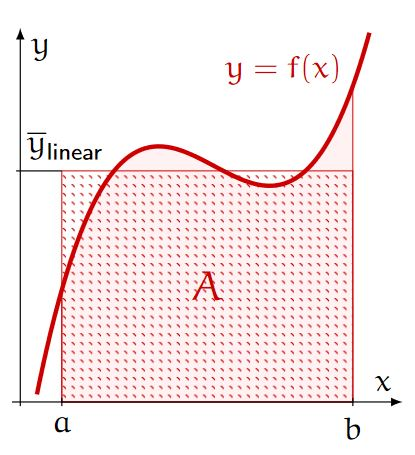
\includegraphics[width=50mm,scale=0.5]{mittelwert}
\end{minipage} \hfill
\begin{minipage}{0.5\textwidth}
    Der lineare Mittlwert $\overline{y}_{linear}$ der Funktion $y=f(x)$
    über dem Intervall $[a,b]$ gibt an, welchen Wert diese Funktion im Mittel hat. \\
    Die Fläche des Rechtecks der Höhe $\overline{y}$ ist gleich der Fläche der Kurve
    $y=f(x)$ \\
    $A = \overline{y}_{linear}(b-a) = \int\limits_a^bf(x)dx$
\end{minipage}

\subsection{Theorem - lineare Mittelwert}
Der lineare Mittelwert von $f$ über $[a,b]$: $\overline{y}_{linear} = \frac{1}{b-a}\int\limits_a^bf(x)dx$

\subsection{Beispiel}
Berechne den linearen Mittelwert der Funktion $y=\ln x$ im Intervall $[1,5]$ \\
$\overline{y}_{linear} = \frac{1}{5-1}\int\limits_1^5\ln xdx$
$ = \frac{1}{4}\left[ x(\ln x)\right]_1^5 = \frac{1}{4}(5(\ln 5-1))-1(0-1) \approx 1.012$

\subsection{Theorem - quadratische Mittelwert}
Der quadratische Mittelwert von $y=f(x)$ über dem Intervall $[a,b]$ ist definiert durch: \\
$\overline{y}_{quadratisch} = \sqrt{\frac{1}{b-a}\int\limits_a^b[f(x)]^2dx}$ \\

Sowohl lineare wie auch quadratische Mittelwerte werden oft im Zusammenhang
mit periodischen Funktionen verwendet. In diesem Fall ist das Intervall $[a,b]$
meist ein Intervall von der Länge einer Periode $T$. Dabei ist es egal, welches
der unendlich vielen Intervalle mit dieser Eigenschaft verwendet wird.
Meist verwendet man deshalb das Intervall $[0,T]$.

\subsection{Theorem - Mittelwertsatz der Integralrechnung}
Ist $f$ auf dem Intervall $[a,b]$ stetig, dann gibt es einen Punkt $\epsilon \in [a,b]$ 
so, dass gilt: \\
$f(\epsilon)(b-a)=\int\limits_a^bf(x)dx$

\end{document}